\chapter{Background}
\label{ch:background}

%%%%%%%%%%%%%%%%%%%%%%%%%%%%%%%%%%%%%%%%%%%%%%%%%
% ANOMALY DETECTION
%%%%%%%%%%%%%%%%%%%%%%%%%%%%%%%%%%%%%%%%%%%%%%%%%
\section{Anomaly detection}
\label{sec:anomalyDetection}
Anomaly detection is the process of detecting patterns in a given data set that 
do not conform to an established normal behavior \cite{Chandola:2007}. The terms
`anomaly' and `outlier' are used synonymously, both within this thesis and more 
generally in the field of statistics. According to \citeauthor{Hawkins:1980} 
\cite{Hawkins:1980}:

% TODO: some sort of formatting
\begin{quote}
An outlier is an observation which deviates so much from the other observations 
as to arouse suspicions that it was generated by a different mechanism.
\end{quote}

The importance of anomaly detection is due to the fact that anomalies in data
translate to significant (and often critical) actionable information in a wide 
variety of application domains \cite{Chandola:2007}.

% WHAT ARE ANOMALIES?
\subsection{What are anomalies?}
\label{sec:whatAreAnomalies}
Anomalies are patterns in data that do not conform to a well defined notion of
normal behavior. \hyperref[fig:2d-anomalies]{Figure~\ref{fig:2d-anomalies}} 
illustrates anomalies in a simple 2-dimensional data set. The data has two 
normal regions, $N_{1}$ and $N_{2}$, since most observations lie in these two 
regions. Points that are sufficiently far away from the regions, such as points 
$o_{1}$ and $o_{2}$, and points in region $O_{3}$, are considered to be 
anomalies.

\begin{figure}
\centering
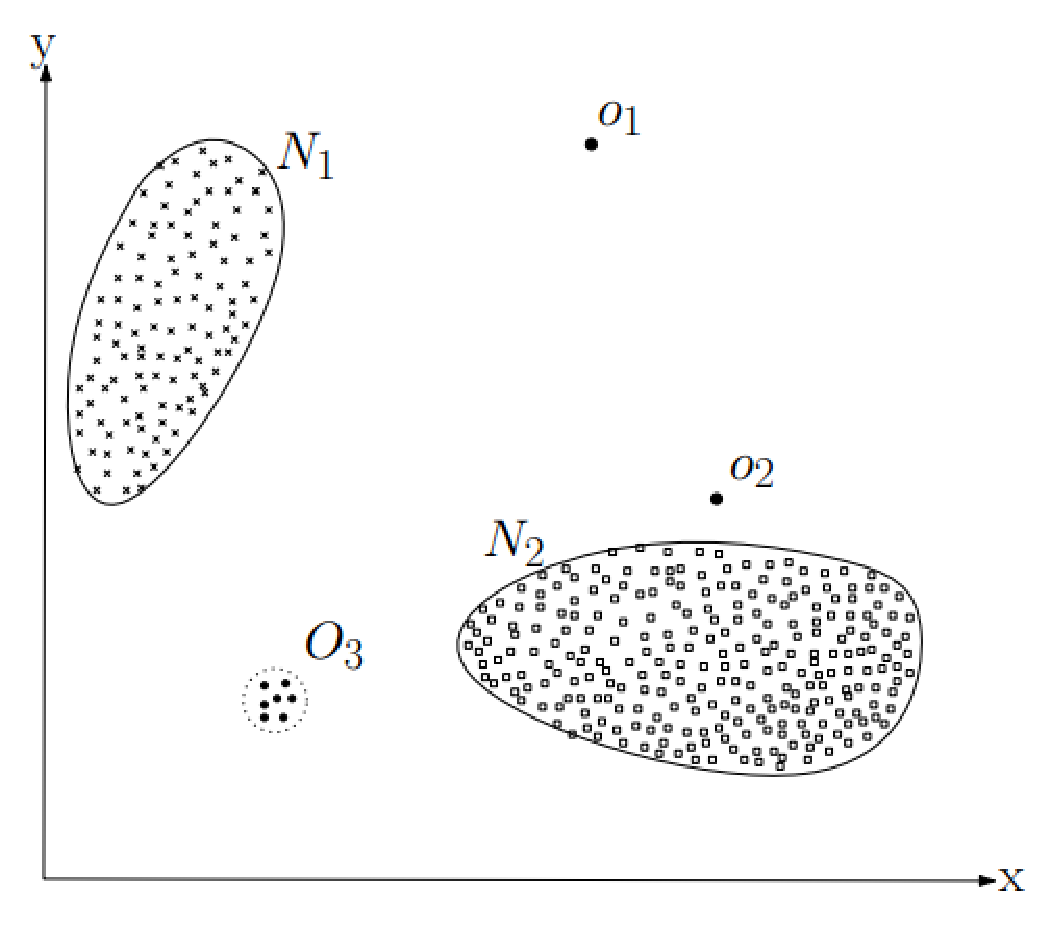
\includegraphics[width=0.5\textwidth]{2d-anomalies}
\caption[A simple example of anomalies in a 2-dimensional data set.]{A simple 
example of anomalies in a 2-dimensional data set \cite{Chandola:2007}.}
\label{fig:2d-anomalies}
\end{figure}

% CHALLENGES
\subsection{Challenges}
\label{sec:anomalyDetectionChallenges}
At an abstract level, an anomaly is defined as a pattern that does not conform 
to expected normal behavior \cite{Chandola:2007}. A straightforward anomaly 
detection approach, therefore, is to define a region representing normal 
behaviour and declare any observation in the data which does not belong to this 
normal region as an anomaly. But several factors make this apparently simple 
approach very challenging:

\begin{itemize}
\item Defining a normal region which encompasses every possible normal behaviour 
is very difficult. In addition, the boundary between normal and anomalous 
behaviour is often not precise. Thus an anomalous observation which lies close
to the boundary can actually be normal, and vice-versa.
\item When anomalies are the result of malicious actions, the malicious 
adversaries often adapt themselves to make the anomalous observations appear 
like normal, thereby making the task of defining normal behavior more difficult.
\item In many domains normal behavior keeps evolving and a current notion of
normal behavior might not be sufficiently representative in the future.
\item The exact notion of an anomaly is different for different application 
domains. For example, in the medical domain a small deviation from normal (for
example, fluctuations in body temperature) might be an anomaly, while similar 
deviation in the stock market domain (for example, fluctuations in the value of 
a stock) might be considered as normal. Thus applying a technique developed in 
one domain to another is not straightforward.
\item Availability of labeled data for training/validation of models used by 
anomaly detection techniques is usually a major issue.
\item Often the data contains noise which tends to be similar to the actual 
anomalies and hence is difficult to distinguish and remove.
\end{itemize}

Due to the above challenges, the anomaly detection problem, in its most general
form, is not easy to solve. In fact, most of the existing anomaly detection 
techniques solve a specific formulation of the problem. The formulation is 
induced by various factors such as nature of the data, availability of labeled 
data, type of anomalies to be detected, etc. Often, these factors are determined
by the application domain in which the anomalies need to be detected. 
Researchers have adopted concepts from diverse disciplines such as statistics, 
machine learning, data mining, information theory, spectral theory, and have 
applied them to specific problem formulations.

% CLASSIFICATION
\subsection{Classification}
\label{sec:anomalyClassification}
In general, two different kinds of outliers exist: global outliers and local 
outliers. Global outliers are distinct with respect to the whole data set, while
local outliers are distinct with respect to data points in their local 
neighbourhood \cite{Vries:2011}. The task of global outlier detection has 
undergone much research \citeneeded{}, but this has not been the case for local 
outlier detection. In the paper \citetitle{Vries:2011}, \citeauthor{Vries:2011} 
optimise the use of local outlier factor (LOF) for large and high-dimensional 
data and propose projection-indexed nearest-neighbours (PINN) --- a novel 
technique that exploits extended nearest-neighbour sets in a reduced-dimensional
space --- to create an accurate approximation for k-nearest-neighbour distances, 
which is used as the core density measurement within LOF \cite{Vries:2011}.

\subsection{Types of anomalies}
\label{sec:typesOfAnomalies}
Anomalies can be classified into three categories \cite{Chandola:2007}:

\begin{description}
\item[Point anomaly] If an individual data instance can be considered as 
anomalous with respect to the rest of data, then the instance is termed as a 
point anomaly. This is the simplest type of anomaly. Referring to 
\hyperref[fig:2d-anomalies]{Figure~\ref{fig:2d-anomalies}}, points $o_{1}$ and 
$o_{2}$, as well as all points in region $O_{3}$ lie outside the boundary of the
normal regions, and are hence point anomalies.

\item[Contextual anomalies] If a data instance is anomalous in a certain 
context, but not otherwise, then it is termed a contextual anomaly. The notion 
of a context is induced by the structure in the data set and has to be specified
as part of the problem formulation.

\begin{figure}
\centering
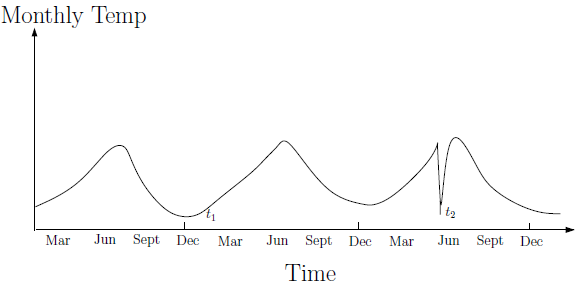
\includegraphics[width=0.5\textwidth]{contextual-anomalies}
\caption[Contextual anomaly $t_{2}$ in a temperature time series.]{Contextual 
anomaly $t_{2}$ in a temperature time series. Note that the temperature at time 
$t_{1}$ is same as that at time $t_{2}$ but occurs in a different context and 
hence is not considered as an anomaly \cite{Chandola:2007}.}
\label{fig:contextual-anomalies}
\end{figure}

Contextual anomalies have been most commonly explored in time-series data and 
spatial data. \hyperref[fig:contextual-anomalies]
{Figure~\ref{fig:contextual-anomalies}} shows one such example for a temperature
time series which shows the monthly temperature of an area over last few years. 
A temperature of $35\degree F$ might be normal during the winter (at time 
$t_{1}$) at that place, but the same value during summer (at time $t_{2}$) would
be an anomaly.

\item[Collective anomalies] If a collection of related data instances is 
anomalous with respect to the entire data set, it is termed as a collective 
anomaly. The individual data instances in a collective anomaly may not be 
anomalies by themselves, but their occurrence together as a collection is 
anomalous. \hyperref[fig:collective-anomalies]
{Figure~\ref{fig:collective-anomalies}} illustrates an example which shows a 
human electrocardiogram output. The highlighted region denotes an anomaly 
because the same low value exists for an abnormally long time. Note that that 
low value by itself is not an anomaly.

\begin{figure}
\centering
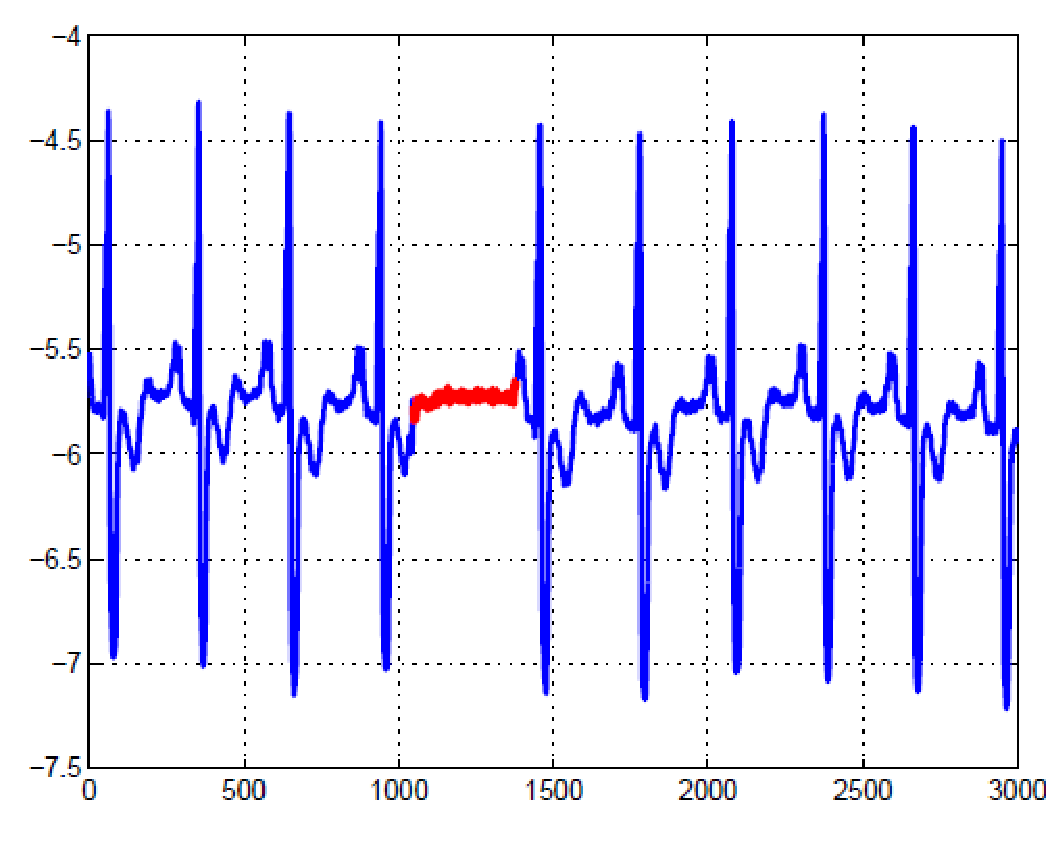
\includegraphics[width=0.5\textwidth]{collective-anomalies}
\caption[Collective anomaly corresponding to an \emph{Atrial Premature 
Contraction} in an human electrocardiogram output.]{Collective anomaly 
corresponding to an \emph{Atrial Premature Contraction} in an human 
electrocardiogram output \cite{Goldberger:2000}.}
\label{fig:collective-anomalies}
\end{figure}

\end{description}

% APPROACHES
\subsection{Approaches}

\begin{description}
\item[Classical] A point is declared to be an outlier if its distance from the 
mean is sufficiently large.
\item[Principal Component Analysis] An outlier is usually declared if the point 
is sufficiently far away from the subspace spanned by the eigenvectors 
corresponding to the highest eigenvalues.
\item[Distance based] A point can be declared to be an outlier if its distance 
to its kth nearest-neighbour is sufficiently large.
\item[Statistical based] Statistical methods are often model-based and assume 
that the data should follow some distribution. With knowledge of the 
distribution, data point are evaluated by their fitness to the assumed 
distribution. If the probability of a data instance is less than a certain 
threshold, then that data point is considered an anomaly.
\end{description}

Although distance is an effective non-parametric approach to detecting outliers,
the drawback is the amount of computation time required. Straightforward 
algorithms, such as those based on nested loops, typically require $O(N^{2})$
distance computations. This quadratic scaling means that it will be very 
difficult to mine outliers as we tackle increasingly larger data sets. This is a 
major problem for many real databases where there are often millions of records 
\cite{Bay:2003}.

\subsubsection{Distance based}
In this approach, one looks at the local neighborhood of points for an example 
typically defined by the $k$ nearest examples (also known as neighbours). If the
neighbouring points are relatively close, then the example is considered normal;
if the neighbouring points are far away, then the example is considered unusual.
The advantages of distance-based outliers are that no explicit distribution 
needs to be defined to determine unusualness, and that it can be applied to any 
feature space for which we can define a distance measure \cite{Bay:2003}.

Researchers have tried a variety of approaches to find these outliers 
efficiently. The simplest are those using nested loops \cite{Bay:2003}. In the 
basic version one compares each example with every other example to determine 
its $k$ nearest neighbors. Given the neighbors for each example in the data set,
simply select the top $n$ candidates according to the outlier definition. This 
approach has quadratic complexity as we must make all pairwise distance 
computations between examples.

Another method for finding outliers is to use a spatial indexing structure such 
as a KD-tree, R-tree, or X-tree to find the nearest neighbors of each candidate 
point. One queries the index structure for the closest $k$ points to each 
example, and as before one simply selects the top candidates according to the 
outlier definition. For low-dimensional data sets this approach can work 
extremely well and potentially scales as $O(N \log N)$ if the index tree can
find an example's nearest neighbors in $\log N$ time. However, index structures 
break down as the dimensionality increases \cite{Bay:2003}.

\subsubsection{Statistical based}
A common distribution considered when modelling data is the `Normal' 
distribution. Using this model, the probability that a data instance lies within
$k$ standard deviations $\sigma$ from the mean $\mu$ is the area between 
$\mu - k\sigma$ and $\mu + k\sigma$.

% LOCAL OUTLIER FACTOR
\subsection{Local Outlier Factor}
\label{sec:localOutlierFactor}
`Local Outlier Factor' is a formula that captures the degree to which a data 
point is an outlier with respect to its local neighbourhood. In this context,
`local' means that the determination of the data points does not depend on 
knowledge of the global distribution of the data set.

%%%%%%%%%%%%%%%%%%%%%%%%%%%%%%%%%%%%%%%%%%%%%%%%%
% VECTORS AND MATRICES
%%%%%%%%%%%%%%%%%%%%%%%%%%%%%%%%%%%%%%%%%%%%%%%%%
\section{Vectors and Matrices}
\label{sec:vectorsAndMatrices}

% EIGENVECTORS AND EIGENVALUES
\subsection{Eigenvectors and Eigenvalues}
\label{sec:eigenvectorsAndEigenvalues}
This section will briefly recall some basic definitions of eigenvectors and
eigenvalues, as well as some of their basic properties.

A vector $\mathbf{v}$ is an eigenvector of a matrix $M$ of eigenvalue $\lambda$ 
if:
\begin{displaymath}
M\mathbf{v} = \lambda\textbf{v}
\end{displaymath}

If $\mathbf{v_{1}}$ is an eigenvector of $M$ of eigenvalue $\lambda_{1}$, 
$\mathbf{v_{2}}$ is an eigenvector of $M$ of eigenvalue $\lambda_{2} \neq 
\lambda_{1}$, and $M$ is symmetric, then $\mathbf{v_{1}}$ is orthogonal to 
$\mathbf{v_{2}}$.

For a symmetric matrix $M$, the multiplicity of an eigenvalue $\lambda$ is the
dimension of the space of eigenvectors of eigenvalue $\lambda$. Also recall that
every $n{\times}n$ symmetric matrix has $n$ eigenvalues, counted with 
multiplicity. Thus, it has an orthonormal basis of eigenvectors, 
$\begin{Bmatrix} \mathbf{v_{1}} & \ldots & \mathbf{v_{n}} \end{Bmatrix}$ with
eigenvalues $\lambda_{1} \leq \lambda_{2} \leq \ldots \leq \lambda_{n}$ so that:
\begin{displaymath}
M\mathbf{v_{i}} = \lambda_{i}\mathbf{v_{i}} \quad \forall i
\end{displaymath}

If we let $V$ be the matrix whose $i$th column is $v_{i}$ and $\Lambda$ be the 
diagonal matrix whose $i$th diagonal is $\lambda_{i}$, we can write this more 
compactly as:
\begin{displaymath}
MV = V\Lambda
\end{displaymath}

Multiplying by $V^{T}$ on the right, we obtain the eigen-decomposition of $M$:
\begin{displaymath}
M = MVV^{T} = V{\Lambda}V^{T} = \sum_{i} \lambda_{i}\mathbf{v_{i}}\mathbf{v_{i}^{T}}
\end{displaymath}

% EIGEN DECOMPOSITION
\subsection{Eigen decomposition}
\label{sec:eigenDecomposition}
% TODO

% LAPLACIAN MATRICES
\subsection{Laplacian Matrices}
\label{sec:laplacianMatrices}
\nocite{Berkeley:1999}
\nocite{Pati:2011}
\nocite{Spielman:2006}
Recall that a weighted, undirected graph $G = (V,E,w)$ is essentially an 
undirected graph $G = (V,E)$ along with a function $w : E \rightarrow 
\Re^{+}$, where $\Re^{+}$ denotes the set of positive real numbers.

The adjacency matrix of a weighted graph $G$ will be denoted $A_{G}$, and is
given by:
\begin{displaymath}
A_{G}(i,j) := 
    \left\{
        \begin{array}{ll}
            \mathit{w}(i,j) &   \quad \text{if $(i,j) \in E$} \\
            0 &                 \quad \text{otherwise}
        \end{array}
    \right.
\end{displaymath}

The degree matrix of a weighted graph $G$ will be denoted $D_{G}$, and is the
diagonal matrix such that:
\begin{displaymath}
D_{G}(i,i) = \sum_{j} A_{G}(i,j)
\end{displaymath}

A Laplacian Matrix is a matrix representation of a graph, defined by the
equation:
\begin{displaymath}
L_{G} = D_{G} - A_{G}
\end{displaymath}

Now, let $G_{1,2}$ be a graph on two vertices with a single edge of weight $1$.
\begin{displaymath}
L_{G_{1,2}} :=
    \begin{bmatrix}
        1 & -1 \\
        -1 & 1
    \end{bmatrix}
\end{displaymath}

For the graph with $n$ vertices and just one edge between vertices $u$ and $v$, 
we can define the Laplacian Matrix similarly. For concreteness, I'll call this
graph $G_{u,v}$. It's Laplacian Matrix is the $n{\times}n$ matrix whose only 
non-zero entries are in the intersections of rows and columns $u$ and $v$. The 
$2{\times}2$ matrix at the intersections of these rows and columns is, of 
course:
\begin{displaymath}
    \begin{bmatrix}
        1 & -1 \\
        -1 & 1
    \end{bmatrix}
\end{displaymath}

For a weighted graph $G = (V,E,w)$, we define:
\begin{displaymath}
L_{G} := \sum_{(u,v) \in E} w(u,v)L_{G_{u,v}}
\end{displaymath}

\paragraph{Properties}
For a graph $G$ and its Laplacian Matrix $L$ with eigenvalues $\lambda_{0} < 
\lambda_{1} < \ldots < \lambda_{n-1}$:

\begin{itemize}
\item $L$ is a symmetric matrix. This means the eigenvalues of $L$ are real, and
its eigenvectors are real and orthogonal.
\item $L$ is always positive-semidefinite ($\forall i, \lambda_{i} \geq 0; 
\lambda_{0} = 0$).
\item Let $G = (V,E)$ be a graph, and let $0 = \lambda_{1} \leq \lambda_{2}
\leq \ldots \leq \lambda_{n}$ be the eigenvalues of its Laplacian Matrix. Then, 
$\lambda_{2} > 0$ if and only if $G$ is connected.
\item The number of times $0$ appears as an eigenvalue in the Laplacian Matrix 
is the number of connected components in the graph.
\item $\lambda_{0}$ is always $0$ because every Laplacian Matrix has an 
eigenvector of $\begin{bmatrix} 1 & 1 & \ldots & 1 \end{bmatrix}$ that, for each
row, adds the corresponding node's degree to a ``-1'' for each neighbour, 
thereby producing zero by definition.
\item The smallest non-zero eigenvalue of $L$ is called the spectral gap.
\item If we arbitrarily assign an orientation to the edges in $G$ and label each
edge, then we can define the vertex edge incidence matrix $Q$ by:
\begin{displaymath}
Q_{ij} := 
    \left\{
        \begin{array}{ll}
            1 &     \quad \text{if $e_{j}$ starts from $i$} \\
            -1 &    \quad \text{if $e_{j}$ ends at $i$} \\
            0 &     \quad \text{otherwise}
        \end{array}
    \right.
\end{displaymath}
Then the Laplacian Matrix $L$ satisfies $L = Q^{T}Q$, regardless of the 
orientation of the edges.
\item The second smallest eigenvalue of $L$ ($\lambda_{2}$) is the algebraic 
connectivity of $G$. $\lambda_{2} > 0$ if and only if $G$ is connected.
\end{itemize}

%%%%%%%%%%%%%%%%%%%%%%%%%%%%%%%%%%%%%%%%%%%%%%%%%
% COMMUTE TIME
%%%%%%%%%%%%%%%%%%%%%%%%%%%%%%%%%%%%%%%%%%%%%%%%%
\section{Commute Time}
\label{sec:commuteTime}

% INTRODUCTION
\subsection{Introduction}
\label{sec:commuteTimeIntroduction}
Commute time is a robust distance metric derived from a random walk on graphs 
\cite{Khoa:2012}. In \citetitle{Khoa:2012}, \citeauthor{Khoa:2012} demonstrated 
how commute time can be used as a distance measure for data mining tasks such as
anomaly detection and clustering. A prohibitive limitation of this technique is 
that the calculation of commute time involves the eigen decomposition of the 
graph Laplacian, making it impractical for large graphs.

A major advantage of using commute time as a distance metric for outlier 
detection is that it effectively captures not only the distances between data 
points but also the density of the data \citeneeded{}. This property results in 
a distance metric that can be effectively used to capture global, local and 
group anomalies.

The commute time between two nodes $i$ and $j$ in a graph is the number of steps
that a random walk, starting from $i$ will take to visit $j$ and then come back 
to $i$ for the first time. The fact that the commute time is averaged over all 
paths (and not just the shortest path) makes it more robust to data 
perturbations and it can also capture graph density \cite{Khoa:2012}. Since it 
is a measure which can capture the geometrical structure of the data and is 
robust to noise, commute time can be applied in methods where Euclidean or other
distances are used and thus the limitations of these metrics can be avoided.

% LIMITATIONS
\subsection{Limitations}
\label{sec:commuteTime:limitations}
The computation of commute time requires the eigen decomposition (see 
\hyperref[sec:eigenDecomposition] {Section~\ref{sec:eigenDecomposition}}) of the
graph Laplacian matrix (see \hyperref[sec:laplacianMatrices] 
{Section~\ref{sec:laplacianMatrices}}), a computation which takes $O(n^{3})$ 
time and thus is not practical for large graphs \citeneeded{}. Methods to 
approximate the commute time to reduce the computational time are required in 
order to efficiently use commute time in large datasets.

% ANOMALY DETECTION USING COMMUTE TIME
\subsection{Anomaly Detection Using Commute Time}
\label{sec:anomalyDetectionUsingCommuteTime}
% TODO

%%%%%%%%%%%%%%%%%%%%%%%%%%%%%%%%%%%%%%%%%%%%%%%%%
% DISTANCE METRICS
%%%%%%%%%%%%%%%%%%%%%%%%%%%%%%%%%%%%%%%%%%%%%%%%%
\section{Distance metrics}
\label{sec:distanceMetrics}
Distance is a quantitative description of how far apart two objects are. 
Mathematically, a distance or metric is a function describing how close or far 
away data points in some space are from each other \cite{Khoa:2012}.

% EUCLIDEAN DISTANCE
\subsection{Euclidean distance}
\label{sec:euclideanDistance}
An Euclidean distance between two data points in a space is the norm of the 
difference between two vectors corresponding to these data points 
\cite{Khoa:2012}. Euclidean distance is extremely sensitive to the scale of the 
features involved. When dealing with features of vastly different scales, the 
effects of the larger feature dominant over the smaller feature in terms of the 
Euclidean distance. This problem is usually solved by normalizing the data 
values. Another issue, however, with Euclidean distance is that it is unable to 
take into account any correlation between data features.

% MAHALANOBIS DISTANCE
\subsection{Mahalanobis distance}
\label{sec:mahalanobisDistance}
Mahalanobis distance is a distance measure that considers the covariance between
data features. Mahalanobis distance, however, is extremely sensitive to 
anomalies as anomalies affect both the mean and the covariance of the data.

% GRAPH GEODESIC DISTANCE
\subsection{Graph geodesic distance}
\label{sec:graphGeodesicDistance}
% TODO

%%%%%%%%%%%%%%%%%%%%%%%%%%%%%%%%%%%%%%%%%%%%%%%%%
% MARKOV CHAINS
%%%%%%%%%%%%%%%%%%%%%%%%%%%%%%%%%%%%%%%%%%%%%%%%%
\section{Markov chains}
\label{sec:markovChains}
A `Markov chain' is a chance process in which the outcome of a given experiment 
can affect the outcome of the next experiment \cite{Grinstead:1997}. For a 
Markov chain, we have a set of states $S = \left\{ s_{1}, s_{2}, \ldots, s_{r} 
\right\}$ with a process starting in one of the states and moving from state 
$s_{i}$ to $s_{j}$ with a probability $p_{ij}$ not dependent upon which states 
the chain was in before the current state. The probabilities $p_{ij}$ are called
\emph{transition probabilities}, and the complete matrix $\mathbf{P}$ of 
probabilities is known as the \emph{transition matrix}.

The probability that, given the chain is in state $i$ now, it will be in state 
$j$ in two steps is denoted by $p_{ij}^{(2)}$. In general, if a Markov chain has 
$r$ states, then:

\begin{displaymath}
p_{ij}^{(2)} = \sum_{k=1}^{r} p_{ik}p{kj}
\end{displaymath}

%%%%%%%%%%%%%%%%%%%%%%%%%%%%%%%%%%%%%%%%%%%%%%%%%
% RANDOM PROJECTIONS
%%%%%%%%%%%%%%%%%%%%%%%%%%%%%%%%%%%%%%%%%%%%%%%%%
\section{Random projections}
\label{sec:randomProjections}
% TODO

%%%%%%%%%%%%%%%%%%%%%%%%%%%%%%%%%%%%%%%%%%%%%%%%%
% RANDOM WALKS ON GRAPHS
%%%%%%%%%%%%%%%%%%%%%%%%%%%%%%%%%%%%%%%%%%%%%%%%%
\section{Random walks on graphs}
\label{sec:randomWalks}

Assume we are given a connected undirected and weighted graph $G = (V,E,W)$ with
edge weights $(w_{ij})_{i,j \in V} >= 0$ be the graph adjacency matrix. A degree
of a node $i$ is $d_{i} = \sum_{j \in N(i)} w_{ij}$ where $N(i)$ is a set of 
neighbours of node $i$. All nodes nonadjacent to $i$ are assumed to have a 
weight of $w_{ij} = 0$.

A random walk is a sequence of nodes on a graph visited by a random walker: 
starting from a node, the random walker moves to one of its neighbours with some
probability. Then from that node, it proceeds to one of its own neighbours with 
some probability, and so on \cite{Khoa:2012}. The random walk is a finite Markov
chain that is time-reversible, which means the reverse Markov chain has the same
transition probability matrix as the original Markov chain \cite{Lovasz:1996}.

The probability that a random walker selects a particular node from is 
neighbours is determined by the edge weights of the graph. The larger the weight
${w_ij}$ of the edge connecting nodes $i$ and $j$, the more often the random 
walker travels through that edge.

%%%%%%%%%%%%%%%%%%%%%%%%%%%%%%%%%%%%%%%%%%%%%%%%%
% NEAREST NEIGHBOUR ALGORITHMS
%%%%%%%%%%%%%%%%%%%%%%%%%%%%%%%%%%%%%%%%%%%%%%%%%
\section{Nearest Neighbour Algorithms}
\label{sec:nearestNeighbourAlgorithms}
% TODO

%%%%%%%%%%%%%%%%%%%%%%%%%%%%%%%%%%%%%%%%%%%%%%%%%
% SOLVERS
%%%%%%%%%%%%%%%%%%%%%%%%%%%%%%%%%%%%%%%%%%%%%%%%%
\section{Solvers}
\label{sec:solvers}

% SPIELMAN-TENG SOLVER
\subsection{Spielman-Teng Solver}
\label{sec:spielmanTengSolver}
\nocite{Spielman:2006}
Spielman and Teng presented a randomised algorithm that, on input a symmetric, 
weakly diagonally dominant $n{\times}x$ matrix $A$ with $m$ non-zero entries and
an $n$-vector $\mathbf{b}$, produces an $\tilde{\mathbf{x}}$ such that 
$\begin{Vmatrix} \tilde{\textbf{x}} - A^{\dagger}\textbf{b} \end{Vmatrix}_{A} 
\leq \epsilon \begin{Vmatrix} A^{\dagger}\mathbf{b} \end{Vmatrix}_{A}$ in 
expected time:
\begin{displaymath}
m \log^{O(1)} n \log (1/\epsilon)
\end{displaymath}
